\chapter{Use case}
\label{chap:Frontend}

As a proof of concept, we have integrated our backend with a user interface. 
Originally we planned to build one from scratch, but while doing our research on the state of the art, we stumbled upon several existing alternatives. 
A very interesting one is RDFExplorer, developed by Vargas et al.~\cite{Vargas2019}. 
In their design, Vargas et al. propose a language and a visual interface that allow users to build and execute graph-based queries in an intuitive way. 
Their claim is that their work allows non-expert users to express graph-pattern queries better than existing interfaces with similar expressiveness. 

In this chapter we will focus on the proof of concept of our design: 
providing users query-term suggestions while they are building SPARQL queries. 
That said, while we are using RDFExplorer as our user interface, any user interface that would provide users suggestions for their SPARQL query building process would be a valid candidate.

We will start by describing the RDFExplorer system and some issues it exhibits while providing suggestions, mainly because of the way it gets suggestions directly from the Wikidata endpoint results. 
We will then proceed to describe an integration with our backend API to get better response times while parallelizing access to both our local specialized index and the remote endpoint.

\section{RDFExplorer}

RDFExplorer is a query building interface that allows users to visually create queries by adding entities and properties as they would add nodes and edges in a graph. The following is an example of a query built via RDFExplorer. In it, \texttt{?var1} refers to instances of \texttt{human} with \texttt{place of birth} in \texttt{Honolulu}.

\begin{figure}[h]
    \centering
        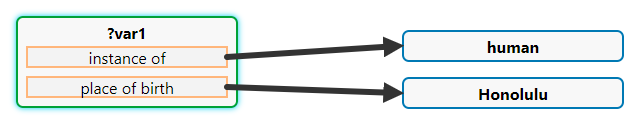
\includegraphics[width=.8\linewidth]{imagenes/rdfExplorer1.png}
        \caption{Building a query with RDFExplorer.}
        \label{fig:rdfExplorer1}
\end{figure}

In the process of building the graph of \Cref{fig:rdfExplorer1}, users can go through the state of \Cref{fig:rdfExplorer_nearTimeout}. 
In this intermediate state neither \textit{place of birth} nor \texttt{Honolulu} are yet given. 
In fact, this might be a very common state in the initial queries built by users, where they construct the graph structure of the query and then look to replace variables with specific constants. 

\begin{figure}[h]
    \centering
        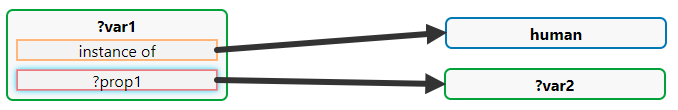
\includegraphics[width=0.8\linewidth]{imagenes/near timeout query.png}
        \caption{Getting suggestions for \texttt{?prop1} takes around 45 seconds on direct queries to the Wikidata Endpoint.}
        \label{fig:rdfExplorer_nearTimeout}
\end{figure}

In order to get results, RDFExplorer will construct a query based on the graph that the user is visually building, send a request to the remote endpoint and await for results: in our case, the Wikidata SPARQL endpoint. 
It is to be noted that this is not the query that is shown in the user interface, but the one that is sent to the endpoint\footnote{As appears in the browser's developer tools}. 
For our example, the graph in \Cref{fig:rdfExplorer_nearTimeout} is represented by the following SPARQL query:

\begin{minted}{SPARQL}
PREFIX wdt: <http://www.wikidata.org/prop/direct/>
PREFIX wd: <http://www.wikidata.org/entity/>
PREFIX wikibase: <http://wikiba.se/ontology#>
PREFIX rdfs: <http://www.w3.org/2000/01/rdf-schema#>
SELECT DISTINCT ?prop1 ?prop1Label WHERE {
  ?var1 ?prop1 ?var2 .
  FILTER isIRI(?var2)
  ?var1 wdt:P31 wd:Q5 .
  ?prop1tmp wikibase:directClaim ?prop1 .
  OPTIONAL {
    ?prop1tmp rdfs:label ?prop1Label .
    FILTER (lang(?prop1Label) = "en")
  }
} LIMIT 10
\end{minted}

One of the issues that users of the current version of RDFExplorer face, is that suggestions directly from the Wikidata remote endpoint can take a long time, or even time out. For example, the suggestions for \textit{?prop1} in \Cref{fig:rdfExplorer_nearTimeout} take around 45 seconds to return, which is not the best user experience while building queries. It is also important to consider that the user might change, add or remove any of the edges and nodes during that time, with which the query will change and be re-sent to the endpoint, resulting in users having no suggestions that allow them to properly explore a dataset. 

In other cases such as in \Cref{fig:rdfExplorer_timeout}, the results will never return if the user asks for suggestions for \texttt{?prop4}, as the underlying query will require a join that generates a very large number of intermediate results. Such queries can be encountered frequently as users will commonly create various nodes to represent the initial structure of their query and then begin to replace variables with the terms they require. 

\begin{figure}[h]
    \centering
        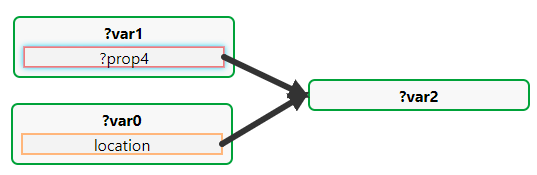
\includegraphics[width=0.7\linewidth]{imagenes/timeout query.png}
        \caption{A timeout query on RDFExplorer.}
        \label{fig:rdfExplorer_timeout}
\end{figure}

One of the issues that our research is trying to solve, in the context of user interfaces such as RDFExplorer, is to enable users to navigate through RDF datasets in almost real-time\footnote{Less than 3 seconds}, while also not limiting the results to 10, but to 100 for backend queries. We do this by approximating results as was seen in \Cref{chap:Backend}.

Our focus during this integration is to compare how different endpoints affect response times. It is not in our focus to make changes to the RDFExplorer interface.

% ##############################################################################################
% ##############################################################################################
% ##############################################################################################

\section{Integration as proof of concept}

In this section we present our backend integration to the RDFExplorer frontend client. The RDFExplorer original source code is currently hosted on github: \url{https://github.com/hvarg/RDFExplorer}. The source code is written in \textit{JavaScript}. We forked this repository\footnote{Forked to \url{https://github.com/gabrieldelaparra/RDFExplorer}} and did our integration in this branch. 

Some code changes were required for our integration: 
\begin{itemize}
    \item Replace the Wikidata endpoint with our local backend.
    \item Replace the request: instead of a SPARQL query, send the graph JSON object.
    \item Convert the response from our backend to the RDFExplorer expected response format.
\end{itemize} 

To get into the details of our integration, we will start by showing the existing architecture of RDFExplorer in \Cref{fig:uiBeforeRequests}. In it, we can see how the system is originally directing its request directly to the Wikidata Endpoint. 

\begin{figure}[h]
    \centering
        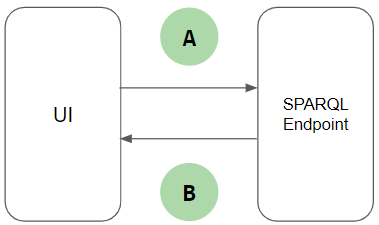
\includegraphics[width=0.4\linewidth]{imagenes/uiBeforeRequest.png}
        \caption{Requests before integration}
        \label{fig:uiBeforeRequests}
\end{figure}

The requests and responses were originally sent as SPARQL queries and the Wikidata API was in charge of returning results as a JSON data object. Both the requests and responses depicted by \texttt{A} and \texttt{B} in \Cref{fig:uiBeforeRequests} are detailed in \Cref{table:uiBeforeRequest}.

\begin{table}[h]
\centering
\begin{tabular}{ll}
Action & Data \\ 
\hline
A              
& \begin{minipage}[t]{0.85\linewidth}
\begin{minted}{SPARQL}
PREFIX ...
SELECT ... 
WHERE {
  ?s ?p ?o .
  FILTER isIRI(?o)
  ?p_tmp wikibase:directClaim ?p .
  OPTIONAL {
    ?p_tmp rdfs:label ?label .
    FILTER (lang(?label) = "en")
  } 
} 
LIMIT 10
\end{minted}
\end{minipage}
\\ \\ \\
B             
& \begin{minipage}[t]{0.85\linewidth}
\begin{minted}{json}
{"head" : 
  { "vars" : 
    [ "prop1", "prop1Label" ] 
  },
"results" : {
  "bindings" : [ {
    "prop1" : {
      "type" : "uri",
      "value" : "http://www.wikidata.org/prop/direct/P611"
    }, 
    // other bindings/variables
  }  ]  }}
\end{minted}
\end{minipage}
\\
\end{tabular}
\caption{UI and Endpoint interactions before our integration.}
\label{table:uiBeforeRequest}
\end{table}

After our integration, the system architecture is as seen in \Cref{fig:uiAfterArchitecture}. It can now be seen that the system directs its requests to our backend, where the requests are parallelized to both our local specialized index and to the remote Wikidata endpoint.

\begin{figure}[h]
    \centering
        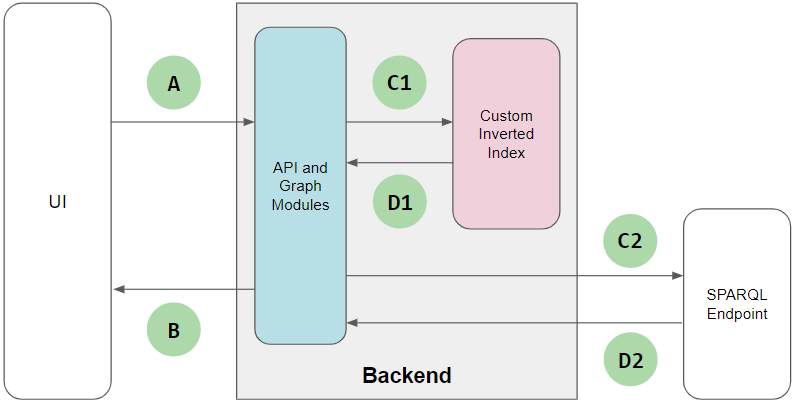
\includegraphics[width=\linewidth]{imagenes/uiAfterRequest.png}
        \caption{Architecture and requests after integration}
        \label{fig:uiAfterArchitecture}
\end{figure}

As can be seen in \Cref{table:uiAfterRequest1} and \Cref{table:uiAfterRequest2}, the requests and responses in this integration have changed. The most important changes are as follows:
\begin{itemize}
    \item \texttt{A:} The UI now sends a JSON object of the query graph.
    \item \texttt{B:} Our response has changed from the original Wikidata response. We now send a different JSON Object.
    \item \texttt{C1} and \texttt{D1} are internal, so no requests and responses are sent; nevertheless, they are shown in the schema for reference.
    \item \texttt{C2:} Is a SPARQL basic graph pattern.
    \item \texttt{D2:} Is the same Wikidata response. The results from either D1 or D2 will be parsed by our system and converted to \texttt{B} depending on the timeouts set and the response times encountered.
\end{itemize}
 
\begin{table}[h]
\centering
\begin{tabular}{ll}
Action & Data \\ 
\hline
A              
& \begin{minipage}[t]{0.85\linewidth}
\begin{minted}{json}
{"nodes": [ {
  "id": 0, "name": "var0",
  "uris": [ ]
  },
  // other nodes
],
"edges": [ {
  "id": 0, "name": "prop0",
  "uris": [],
  "sourceId": 0, "targetId": 1
  },
  // other edges
]}
\end{minted}
\end{minipage}
\\ \\ \\
B             
& \begin{minipage}[t]{0.85\linewidth}
\begin{minted}{json}
{"nodes": [ {
  "id": 0, 
  "suggestions": {
   "Q2": {
     "label": "Earth",
     "uri": "http://www.wikidata.org/entity/Q2"
    }, 
    // other suggestions
    } 
  },
  // other nodes
  ], 
"edges": [ 
  // edges with suggestions
  ]}
\end{minted}
\end{minipage}
\\
\end{tabular}
\caption{UI and Backend interactions after our integration.}
\label{table:uiAfterRequest1}
\end{table}


\begin{table}[h]
\centering
\begin{tabular}{ll}
Action & Data \\ 
\hline
C2             
& \begin{minipage}[t]{0.85\linewidth}
\begin{minted}{SPARQL}
PREFIX ...
SELECT ... 
WHERE {
  ?s ?p ?o .
  FILTER(STRSTARTS(STR(?s), "wd:") .
  FILTER(STRSTARTS(STR(?p), "wdt:") .
  FILTER(STRSTARTS(STR(?o), "wd:") .
} 
LIMIT 100
\end{minted}
\end{minipage}
\\ \\ \\
D2             
& \begin{minipage}[t]{0.85\linewidth}
\begin{minted}{json}
{"head" : 
  { "vars" : 
    [ "prop1", "prop1Label" ] 
  },
  "results" : {
    "bindings" : [ {
      "prop1" : {
        "type" : "uri",
        "value" : "http://www.wikidata.org/prop/direct/P611"
      }, 
    // other bindings/variables
    }  ]  }}
\end{minted}
\end{minipage}
\\
\end{tabular}
\caption{Backend and Endpoint interactions after our integration.}
\label{table:uiAfterRequest2}
\end{table}

Without going into the code nuances for our integration, we rather provide some high-level details on the changes required for our integration. 

Regarding \texttt{A}, originally RDFExplorer sent a SPARQL request to the Wikidata Endpoint, but internally handled a graph object. We considered that using the graph model, which is one step above before the graph-to-SPARQL conversion, could be more flexible for future integrations, so we started our integration there.

The RDFExplorer graph model is a common graph implementation, and also very similar to the one that we are using. In fact, the RDFExplorer implementation has more data values for nodes and edges, which we do not require and thus trimmed for the request. The graph model using for the requests is based on the following structure:
\begin{minted}{json}
{"nodes" : { "id", "uris"[ ], "name" },
 "edges" : { "id", "uris"[ ], "name", "sourceId", "targetId" }}
\end{minted}

Some additional changes, while not required, are that we now check whether the graph  changes during the query construction. Originally, the RDFExplorer UI will send a new request for any changes in the node/edge coordinates or selection. While this is not required, it improves the overall performance since changes to the nodes positions do not trigger a new request now. 

The response that we return in \texttt{B} has also changed. Initially RDFExplorer is waiting for a JSON response from Wikidata. Our integration response will include all the data required by the UI, but with some changes in the structure. 

The response from our system is as follows:
\begin{minted}{json}
{"nodes": { "id", "values": [ { "uri", "label" }, ... ], ... },
 "edges": { "id", "values": [ { "uri", "label" }, ... ], ... }}
\end{minted}

With these changes in place, our RDFExplorer client can now query to our local endpoint and give users suggestions while building SPARQL queries in the graph-based user interface.

The remaining \texttt{C2} and \texttt{D2} work just as they had previously worked from Wikidata to the UI, but this time, the requests and responses are handled by our backend and converted from and to the previously mentioned data structures.

As was mentioned in \Cref{chap:execution}, we will send two queries to both indexes: via \texttt{C1} to our local index and via \texttt{C2} to the remote endpoint. If we receive a response from the remote endpoint (\texttt{D2}) within a configurable timeout threshold, we return these remote endpoint exact results, otherwise if the remote endpoint times out, we return our local approximated results (\texttt{D1}).
